\section{Parallelisierung}
\label{sec:parallelpart}
  Im vorherigen Kapitel haben wir die Berechnung der Gravitationskräfte durch Interpolation approximiert. Dadurch konnten wir die Technik \hquad nutzen um den Rechenaufwand des Algorithmus zu 
  beschleunigen.
  Um die absolute Laufzeit aber noch weiter zu reduzieren sind wir an einer parallel arbeitende Variante dieses Algorithmus interessiert. In diesem Kapitel wird ein Ansatz vorgestellt.
  
  Ziel ist es, zunächst einen einfachen Algorithmus zu entwerfen. Daher beschränken wir uns auf Parallelisierung nach dem Message-Passing-Modell unter Verwendung von MPI. Wir können also 
  $p \in \N$ Prozesse starten. Jeder von diesen hat eine eindeutige $id \in \nullhaken{p-1}$ und seinen privaten Speicherbereich. Insbesondere ist in diesem Modell Shared-Memory ausgeschlossen. 
  Außerdem können die Prozesse miteinander kommunizieren um Daten auszutauschen. Die Menge der Prozesse wird im Folgen mit $\Proc$ bezeichnet.

  
  \subsection{Arbeitsverteilung}
  \label{sec:work}
    Damit wir von parallel arbeitenden Prozessen profitieren können, muss die Arbeit möglichst gleichmäßig auf diese Prozesse verteilt werden. Wir folgen, in modifizierter Variante, dem von 
    \citet{distrh2} vorgestellten Cluster-zentrierten Ansatz. 
    Dieser basiert auf dem Grundgedanken, dass für \vorruck ausschließlich Daten zwischen Vater- und Sohnclustern ausgetauscht werden müssen. Um möglichst viel Kommunikation zu sparen, ist es daher
    besonders effektiv, wenn möglichst viele Söhne durch den selben Prozess verarbeitet werden, wie der Vater. Besonders einfach wird das Verteilen der Cluster und das Loadbalancing, wenn wir $p$ als 
    Zweierpotenz $p = 2^q$ wählen. Da dann die Anzahl von Clustern in $T_\Omega^{(q)}$ gerade $p$ entspricht, können wir diese Ebene, zuzüglich der Sohncluster, optimal auf die Prozesse verteilen.
    Wir gehen im Folgenden immer von einer so gewählten Anzahl Prozesse aus.
    
    Um diesen Ansatz auf den Algorithmus zu übertragen, wird in der in \autoref{lst:init} aufgeführten init-Methode die globale Variable $\tcode{SPLIT_DEPTH} = log_2(p) = q$ gesetzt. 
    Außerdem bekommt die Datenstruktur \code{Cluster} einen weiteren Member: \code{int active}. In diesem  wird die $id$ des für dieses Cluster zuständigen Prozesses gespeichert.
    
    Zudem gibt es aber noch Cluster auf den Ebenen $T_\Omega^{<q} := T_\Omega^{(0)},\dots,T_\Omega^{(q-1)}$. Um ein Cluster $C \in T_\Omega^{<q}$ zu klassifizieren nutzt jeder Prozess $P \in \Proc$
    mit $id_P$ zwei Konstanten. Gilt für alle Nachfahren $\tilde C \in sons*(C)$ $C.\tcode{active} \neq id_P$  , wird der Member $C.\tcode{active}$ auf die \code{int}-Konstante \code{inactive} gesetzt. 
    Gibt es aber Nachfahren $\tilde C \in sons*(C)$ mit $C.\tcode{active} = id_P$, so wird der Member $C.\tcode{active}$ statt dessen auf die \code{int}-Konstante \code{semi_active} gesetzt. Inaktive
    Cluster werden während der \vorruck nicht weiter beachtet. 
    
    \begin{figure}[t]
    \begin{subfigure}{0.9\textwidth}
    \begin{lstlisting}[label=lst:parsetup, caption={Für die Verteilung der Cluster auf die Prozesse angepasste \code{_setup}-Methode.}]
void _setup(Cluster *c, int depth){
  if(depth == SPLIT_DEPTH){
    c->active = ++split_count;
  }

  if(depth < MAX_DEPTH){
    _setup_nonLeafCluster(c, depth);
  }

  if(c->active == semi_active){
    if(c->son[0]->active == inactive && c->son[1]->active == inactive){
      c->active = inactive;
    } else{
      if(c->son[0]->active != world.rank && c->son[0]->active != semi_active &&
	 c->son[1]->active != world.rank && c->son[1]->active != semi_active) {
	c->active = inactive;
      }
    }
  }
}
    \end{lstlisting}
    \end{subfigure}
    \end{figure}
    Um diese Einteilung vorzunehmen, wird vorrangig der Code der Methode \code{_setup(...)} (vgl. \autoref{lst:setup}) angepasst. 
    Zudem bekommt der Konstruktor \code{_new_bound_Cluster} einen neuen Parameter um den Member \code{active} aller Cluster zu initialisieren. Für die Konstruktion der Wurzel ist dieser auf
    \code{semi_active} gesetzt. Danach wird durch die Methode \code{_setup_nonLeafCluster(...)} immer der Wert des Vaters an die Söhne weitergegeben.
    Der angepasste Code der \code{_setup}-Methode ist in \autoref{lst:parsetup} aufgeführt.
    
    Zunächst wird überprüft, ob die \code{SPLIT_DEPTH} erreicht wurde. Ist dies der Fall wird der Member \code{active} auf 
    die $id$ des zuständigen Prozesses gesetzt. Dies geschieht einfach durch abzählen. Als nächstes folgt der bereits aus \autoref{lst:setup} bekannte Aufruf, der das Teilen in Sohncluster, das 
    Sortieren der \code{bodies} und die Rekursion beinhaltet. Der letzte Teil wird beim Abbau der Rekursion durchgeführt. Hier wird für eben die Cluster in $T_\Omega^{(<q)}$ überprüft ob diese 
    auf \code{semi-active} bleiben, oder, falls kein Nachfahre aktiv ist, der Member \code{active} auf \code{inactive} gesetzt wird.
    
    Die Idee der semi-aktiven Cluster beruht darauf, die Gestalt der Spalten- bzw. Zeilenmatrizen $V_\tau$ und $W_\sigma$ auszunutzen. Diese werden für Nicht-Blattcluster durch die Transfermatrizen 
    aus den Söhnen konstruiert (vgl. \autoref{sec:approxf}). Während der \vorw werden für ein solches Cluster $C_{semi} \in T_\Omega^{<q}$ die Ersatzmassen nur aus (semi-)aktiven Söhnen
    errechnet. Da diese Cluster für mehrere Prozesse als semi-aktiv gekennzeichnet sind, werden global betrachtet alle Söhne in der \vorw beachtet. Ist eines dieser Cluster Bestandteil
    eines zulässigen Blockes $b_0 = C_{semi} \times C$ oder $b1 = C \times C_{semi}$, so können die Prozesse ihre Berechnungen untereinander austauschen. Somit werden die Definitionen der Matrizen
    $V_\tau$ und $W_\sigma$ aus \autoref{eq:vtau} beziehungsweise \autoref{eq:wsigma} lediglich auf mehrere Prozesse verteilt und die Summation bei Bedarf aus den Teilergebnissen gebildet.
    
    Unter der Voraussetzung, dass alle notwendigen Information für jeden Prozess vorhanden sind, ist die einzige Anpassung der \koppl, dass sich die Auswertung auf (semi-)aktive
    Targetcluster beschränkt. Auch die \ruckw braucht sich lediglich auf (semi-)aktive Cluster beschränken.
    
    Letztlich verteilt sich die Arbeit durch diesen Ansatz sehr natürlich auf die Prozesse. In \autoref{fig:vertblock} ist dies veranschaulicht. Hier ist dies für einen Prozess $P$ mit $id_P = 1$ 
    und $p = 4$ dargestellt, welche Zuständigkeiten sich für die Blöcke des Blockbaumes aus der Aufteilung der Targetcluster ergeben.
    
    \begin{figure}[b]
      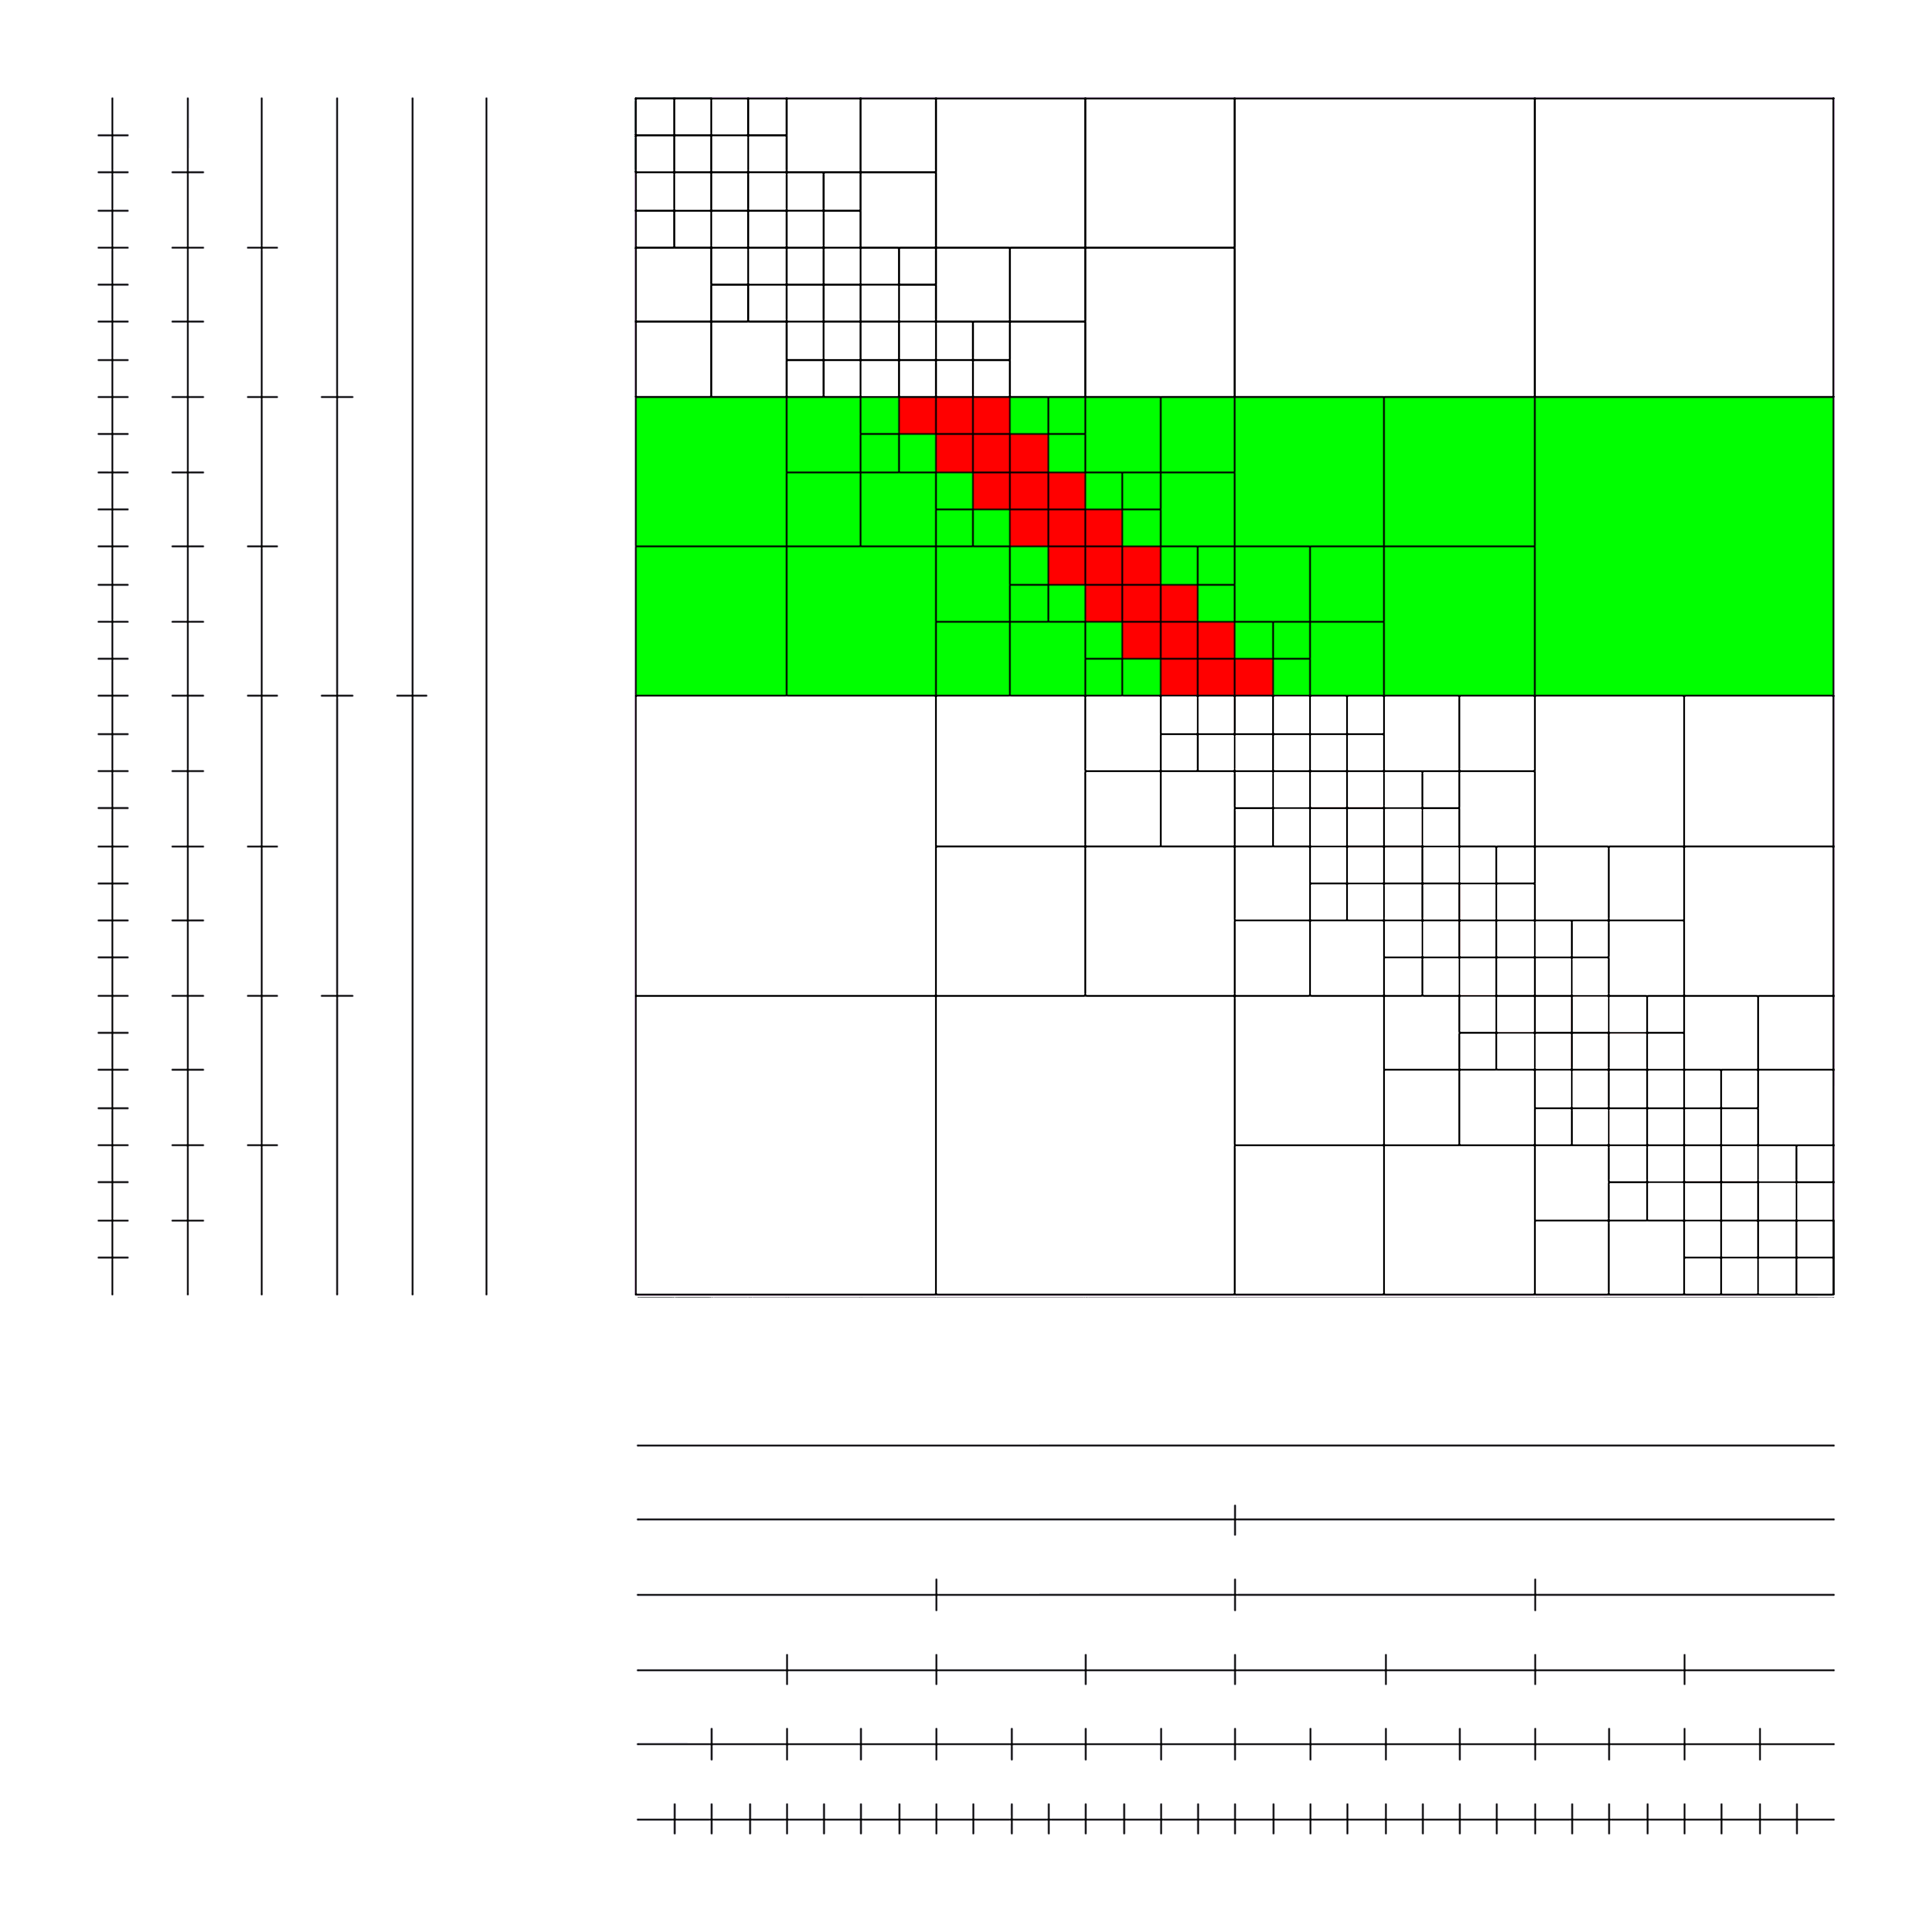
\includegraphics[width=0.8\textwidth]{img/verteilter_blockbaum.png}
      \caption{Für einen Prozess $P$ mit $id_P = 1$ und die Anzahl Prozesse $p = 4$ ist hier die Zuständigkeit des Prozesses $P$ für Blöcke eines Blockbaumes farbig dargestellt.}
      \label{fig:vertblock}
    \end{figure}

    \clearpage
  
  \subsection{Datenverteilung}
  \label{sec:data}
    \TODO{Eine der ersten und grundlegenden Fragen, die bei parallel arbeitenden Programmen geklärt werden muss, ist, wo welche Daten vorhanden sind. Ein Möglicher Ansatz wäre, dass jeder Prozess
    eine Kopie aller Daten hat.}